\documentclass[bakalaurinis.tex]{subfiles}
 
\begin{document}
Čia pateikiamas \textbf{užduočių diagramos} naudojamos darbe apibrėžimas. Tai bus algoritmo rezultato formatas. Siekiama gauti kiek įmanoma tikslesnę užduočių diagramą. Jos komponentai pateikiam \ref{tab:investigated_use_case_diagram_components} lentelėje.

\stepcounter{counter:table:reset}
\begin{center}
    \begin{longtable}{ | p{0.5cm} | p{2cm} |  p{7cm} | c |}
    \caption{\textbf{Užduočių diagramos} komponentai}
	\label{tab:investigated_use_case_diagram_components}
    \\ \hline 
    Nr. & Komponentas & Aprašymas & Žymėjimo pavyzdys\\ 
    \hline 
    \rownumber & Aktorius & Komponentas žymintis sistemos naudotojo tipą. & \vtop{\hbox{\strut }\hbox{\strut 
\includegraphics[width=3cm]{img/use_case_components/actor}}} \\
    \hline
    \rownumber & Vartojimo atvejis & Komponentas specifikuojantis elgsenų aibę, kuri generuoja rezultatą. & \vtop{\hbox{\strut }\hbox{\strut 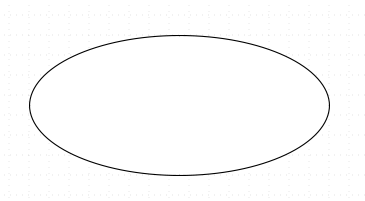
\includegraphics[height=3cm]{img/use_case_components/use_case}}} \\
    \hline
     \rownumber & Asociacija & Komponentas žymintis ryšį tarp aktoriaus ir vartojimo atvejo. & \vtop{\hbox{\strut }\hbox{\strut 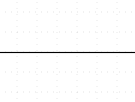
\includegraphics[width=3cm]{img/use_case_components/association}}} \\
    \hline
     \rownumber & Įtraukia & Komponentas žymintis elgseną kuri yra bendra keliems vartojimo atvejams, todėl ji parodoma atskirai nuo jų, kad būtų galima perpanaudoti. & \vtop{\hbox{\strut }\hbox{\strut 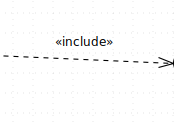
\includegraphics[width=3cm]{img/use_case_components/includes}}} \\
    \hline
    \rownumber & Išplečia & Komponentas žymintis, kad esant tam tikram atvejui vartojimo atvejis įtraukia papildomus vartojimo atvejus. & \vtop{\hbox{\strut }\hbox{\strut 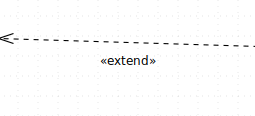
\includegraphics[width=3cm]{img/use_case_components/extend}}} \\
    \hline
    \end{longtable}
\end{center}
\end{document}
